% TEMPLATE for Usenix papers, specifically to meet requirements of
%  USENIX '05
% originally a template for producing IEEE-format articles using LaTeX.
%   written by Matthew Ward, CS Department, Worcester Polytechnic Institute.
% adapted by David Beazley for his excellent SWIG paper in Proceedings,
%   Tcl 96
% turned into a smartass generic template by De Clarke, with thanks to
%   both the above pioneers
% use at your own risk.  Complaints to /dev/null.
% make it two column with no page numbering, default is 10 point

% Munged by Fred Douglis <douglis@research.att.com> 10/97 to separate
% the .sty file from the LaTeX source template, so that people can
% more easily include the .sty file into an existing document.  Also
% changed to more closely follow the style guidelines as represented
% by the Word sample file. 

% Note that since 2010, USENIX does not require endnotes. If you want
% foot of page notes, don't include the endnotes package in the 
% usepackage command, below.

% This version uses the latex2e styles, not the very ancient 2.09 stuff.
\documentclass[letterpaper,twocolumn,10pt]{article}
\usepackage{usenix,epsfig,endnotes,hyperref,soul}
\usepackage{bookmark}
\usepackage{subfigure}
\usepackage{framed}
\usepackage{color}
\usepackage{datetime}
\usepackage{authblk}
\usepackage[nocompress]{cite}

\newcommand{\paa}[1]{{\textcolor{red}{[[#1 -- paa]]}}}
\newcommand{\kam}[1]{{\textcolor{blue}{[[#1 -- kam]]}}}

% If your conference documentclass or package defines these macros,
% change these macros to different names.
\newcommand*{\affaddr}[1]{#1} % No op here. Customize it for different styles.
\newcommand*{\affmark}[1][*]{\textsuperscript{#1}}
\newcommand*{\email}[1]{\texttt{#1}}

\pagenumbering{gobble}

\begin{document}

%don't want date printed
\date{}

%make title bold and 14 pt font (Latex default is non-bold, 16 pt)
\title{\Large \bf LOOM}

\author{
Kamala Ramasubramanian\affmark[1], Ashutosh Raina\affmark[1], Peter Alvaro\affmark[1]\\
\affaddr{\affmark[1]University of California, Santa Cruz}\\
\email{\{kramasub, asraina, palvaro\}@ucsc.edu}
}

\maketitle

% Use the following at camera-ready time to suppress page numbers.
% Comment it out when you first submit the paper for review.
%\thispagestyle{empty}

%%%%%%%%%%%
%     ABSTRACT     %
%%%%%%%%%%%
\subsection*{Abstract}
\input{abstract}

\section{Introduction}
%%%%%%%%%
%     INTRO     %
%%%%%%%%%
Having system traces is useful in order to get high level explanations of system outcomes. 

Not all systems have traces - due to instrumentation and performance overloads. 

All systems generate logs of varying levels of details. 

Can we infer potential causal relationships from logs?

Decompose problem into:
\begin{itemize}
\item Identifying events 
\item Establishing dependencies amongst events
\end{itemize}

If we assume globally unique identifiers at the request level across nodes, the problem of identifying events becomes trivial, but the second problem remains.

If we make the assumption that we are able to run a given workload on a system repeatedly, the key intuition is that the true dependencies of any given event will be present in addition to others. 

We show that we can approach the true set of relationships with a combination of running the system repeatedly and randomly injecting delay on one or more nodes. 


%%%%%%%%%%%%%%%%%%%%%%%
%     BACKGROUND AND MOTIVATION     %
%%%%%%%%%%%%%%%%%%%%%%%
\section{Motivation}
\label{sec:motivation}
Establishing dependencies amongst events is only relevant to distributed executions.
\begin{itemize}
\item Since a total order can be established for events on a single thread of execution
\end{itemize}

The dependencies that we postulate amongst events under consideration should, in the ideal case, be:
\begin{enumerate}
\item Sound:  
All relationships postulated should be true.
\item Complete:
All true relationships should be postulated.
\end{enumerate}

These two requirements are in opposition with each other. 

Two naive approaches:
\begin{enumerate}
\item Events only have dependencies on the same node: 
Sound but not complete. Will miss important dependencies. 

\item Events depend on all preceding events that occurred on a different node: 
Complete but not sound. Will not miss any dependencies, but dependency graph likely to be extremely dense and unrepresentative of truth.
\end{enumerate}

We start with the complete dependency graph and try to make it as sound as possible. 



\section{Background}
Cassandra is an open source NoSQL database designed for high availability of large amounts of data with no single point of failure. [Need citation]

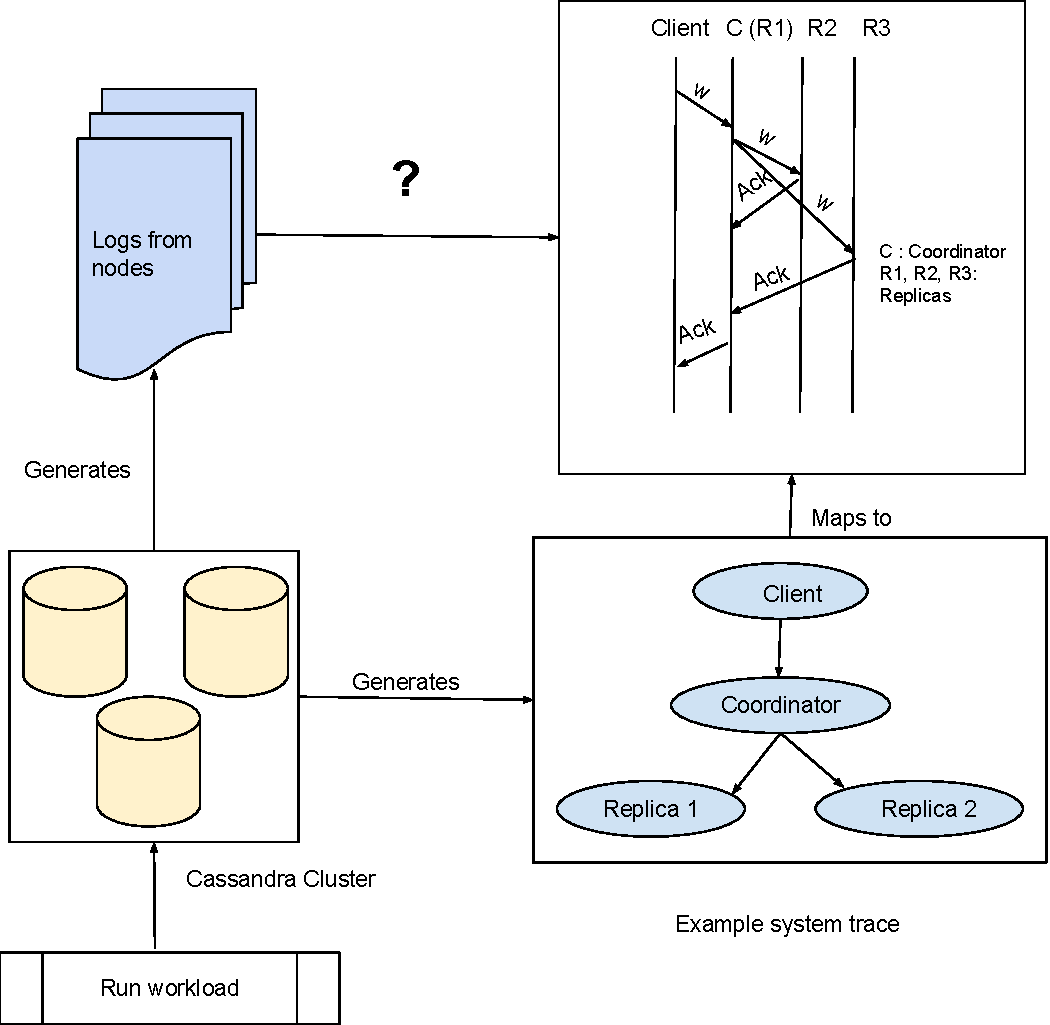
\includegraphics[scale=0.35]{figures/system_model.pdf}

Integration of Zipkin with Cassandra enables us to obtain both the system traces as well as logs from running a query against the database. [Need citation]

We run a single insert query on a replicated cluster and collect both system logs as well as Zipkin traces in JSON format. 

We map the traces obtained to a Lamport diagram of the interaction. The questions we will be addressing are:
\begin{enumerate}
\item Can we reduce the number of dependencies so we can visualize the result?
\item How closely can we approximate the actual interaction?
\end{enumerate}


%%%%%%%%%%%%%%
%     RELATED WORK     %
%%%%%%%%%%%%%%
\begin{enumerate}
\item Mystery machine
\item Lprof
\item Pivot Tracing 
\end{enumerate}


%%%%%%%%%%%%%%%%%%%%%%%%%%%
%    System setup   %
%%%%%%%%%%%%%%%%%%%%%%%%%%%
\section{System setup}
\input{setup_and_intro}

%%%%%%%%%%%%%%%%%%%
%     VISION FOR THE FUTURE     %
%%%%%%%%%%%%%%%%%%%
\section{Future Work}
\begin{enumerate}
\item Identifying events using data mining techniques
\item Strategically introducing delays instead of random delays
\item Moving beyond POC by increasing scale of system and complexity of workload
\end{enumerate}


%%%%%%%%%%%%%
%     CONCLUSION     %
%%%%%%%%%%%%%
%\-\vspace{-1.15cm}
\section{Conclusion}
%\vspace{0.2cm}

%%%%%%%%%%%%%%%%%%
%     ACKNOWLEDGEMENTS     %
%%%%%%%%%%%%%%%%%%
% no ACKs till cameraready
\noindent
%\centerline{\textbf{Acknowledgements}}\\

%\-\vspace{1.5cm}
%%%%%%%%%%%%%
%     REFERENCES     %
%%%%%%%%%%%%%
\nocite{*}
{\footnotesize \bibliographystyle{acm}
\bibliography{references}
}
\end{document}

%%%%%%%%
%       EOF     %
%%%%%%%%

